\documentclass[conference]{IEEEtran}
% \IEEEoverridecommandlockouts % Unneeded: no funding or grant footnote.


\usepackage{cite}
\usepackage{amsmath,amssymb,amsfonts}
\usepackage{algorithmic}
\usepackage{graphicx}
\usepackage{textcomp}
\usepackage{xcolor}
\usepackage{booktabs}
\usepackage{siunitx}
\usepackage{url}
\usepackage{microtype}

\graphicspath{{figures/}}

\def\BibTeX{{\rm B\kern-.05em{\sc i\kern-.025em b}\kern-.08em
    T\kern-.1667em\lower.7ex\hbox{E}\kern-.125emX}}

\begin{document}

\title{Automated Rooftop Solar Pre-Feasibility Assessment from OpenStreetMap Building Footprints}

\author{
\IEEEauthorblockN{1\textsuperscript{st} Oumar Mamoun Ibrahim}
\IEEEauthorblockA{\textit{Department of Computer Engineering} \\
\textit{University of Sharjah}\\
Sharjah, UAE \\
U22200741@sharjah.ac.ae}
\and
\IEEEauthorblockN{2\textsuperscript{nd} Mohamad Khairi bin Ishak}
\IEEEauthorblockA{\textit{Department of Computer Engineering} \\
\textit{University of Sharjah}\\
Sharjah, UAE \\
mishak@sharjah.ac.ae}
}

\maketitle

\begin{abstract}
Rooftop solar photovoltaic (PV) adoption often stalls at the point of first decision, when a business or property owner needs a fast, low-cost feasibility estimate before committing to an engineering study. Existing pre-feasibility methods, including manual satellite-image tracing, light detection and ranging (LiDAR) platforms, and paid application programming interfaces (APIs), are costly, proprietary, or unavailable across much of the United Arab Emirates, the Gulf, and the Global South. Unlike LiDAR platforms such as Google's Project Sunroof, which have little coverage in these regions, this work uses only free, crowdsourced OpenStreetMap (OSM) building-footprint data. This paper presents an open-source Python framework that generates automated rooftop solar feasibility reports from OSM data. Given an address or coordinate, the framework queries the OSM Overpass API for the building polygon, projects it into a local metric frame, and computes footprint area with the shoelace formula. It estimates roof azimuth, applies an irradiance derating factor, and models estimated annual energy yield. Across an empirical validation dataset of 24 diverse buildings in the United Arab Emirates spanning academic, commercial, and industrial typologies, the automated footprint extraction achieves a Mean Absolute Percentage Error (MAPE) of 4.54\% and a coefficient of determination ($R^2$) of 1.000 compared to independent high-resolution satellite measurements. A detailed case study of an academic facility at the University of Sharjah yields an estimated 272.38~kW direct current (DC) array capacity, 260.33~MWh annual generation, and an estimated simple payback period of 2.75 years. Parametric sensitivity analyses demonstrate the scale dependency of perimeter setback buffers and define the operational boundaries where crowdsourced screening is suitable for preliminary decision support.

\end{abstract}

\begin{IEEEkeywords}
Building footprint, geographic information systems, open-source software, OpenStreetMap, photovoltaic pre-feasibility, rooftop solar, solar resource assessment.
\end{IEEEkeywords}

\section{Introduction}

Distributed rooftop solar photovoltaic (PV) systems provide clean on-site electricity, reduce transmission losses, and lower carbon emissions in rapid-growth urban environments. In regions with exceptional solar irradiance, such as the United Arab Emirates (UAE) and the wider Gulf Cooperation Council (GCC), annual global horizontal irradiance (GHI) frequently exceeds 2,000~kWh/m$^2$/year \cite{alhammami2021, hamdi2024}. This resource provides favorable economic fundamentals for commercial, institutional, and residential rooftop generation.

Despite strong technical potential, widespread rooftop solar adoption encounters friction at the initial screening phase. A commercial property owner, facility manager, or residential consumer contemplating solar installation must evaluate technical capacity and financial return before committing capital. However, preliminary engineering site visits conducted by engineering, procurement, and construction (EPC) contractors require physical roof inspections, drone photography, and manual computer-aided drafting (CAD) modeling. These initial surveys cost between \$1,000 and \$5,000 and require multiple weeks to deliver \cite{gassar2021, melius2013}. Consequently, a substantial majority of prospective adopters abandon solar inquiries at this point of first decision.

Commercial software platforms have sought to address this barrier by automating preliminary assessments. Tools such as Google Project Sunroof \cite{gagnon2016} and commercial high-resolution satellite APIs provide instant solar screening. However, these platforms rely on airborne light detection and ranging (LiDAR) and sub-meter aerial photogrammetry. Because airborne LiDAR campaigns require public funding and municipal flight permits, coverage remains concentrated almost exclusively in North America and select Western European countries \cite{rees2025, walch2020}. Across the UAE, the GCC, and most of the Global South, commercial platforms offer zero coverage. Furthermore, commercial solar APIs require ongoing paid subscriptions, software licenses, and cloud connectivity, preventing local deployment by researchers, municipal planners, and small enterprises.

Crowdsourced geospatial data from OpenStreetMap (OSM) provide an alternative foundation for urban spatial modeling \cite{haklay2008}. OpenStreetMap contains millions of volunteer-digitized building footprint polygons worldwide, accessible without licensing fees through public web application programming interfaces (APIs) such as the Overpass API. While previous studies have examined regional building morphologies using OSM \cite{biljecki2020, hecht2013}, existing research either focuses on macro-scale national aggregates in Europe \cite{mainzer2017, assouline2017}, depends on external commercial geographic information system (GIS) software \cite{rees2025}, or models electrical physics without automated geometric extraction \cite{holmgren2018}. Prior literature lacks a lightweight, self-contained, open-source computational pipeline that converts raw street addresses or geographical coordinates directly into verifiable rooftop solar feasibility estimates in a coverage-gap region.

This paper addresses this barrier by making the following specific research contributions:
\begin{enumerate}
    \item \textbf{End-to-End Open Framework:} We implement and document a self-contained Python framework (SolarScan) that executes the complete pre-feasibility workflow: coordinate geocoding, OSM Overpass polygon retrieval, local metric projection, shoelace area computation, perimeter setback buffering, dominant roof azimuth extraction, empirical irradiance derating, system sizing, life-cycle techno-economics, and greenhouse gas carbon offset estimation. The framework operates without commercial GIS licenses, GPU hardware, or paid API keys.
    \item \textbf{Empirical Multi-Building Validation in a Coverage-Gap Region:} We assemble an empirical benchmark of 24 buildings across five UAE Emirates (Sharjah, Dubai, Abu Dhabi, Ajman, and Ras Al Khaimah), evaluating automated OSM extraction against independent sub-meter satellite measurements across academic, commercial, and industrial typologies. We quantify geometric fidelity using Mean Absolute Percentage Error (MAPE), Mean Bias Error (MBE), Root Mean Square Error (RMSE), and correlation coefficients.
    \item \textbf{Sensitivity and Boundary Analysis:} We perform parametric sensitivity analyses on perimeter setback distances and roof orientations, proving analytically that perimeter-based setbacks exhibit strong scale dependency governed by the building's perimeter-to-area ($P/A$) ratio. We define explicit boundaries for when crowdsourced footprint screening is reliable for first-decision feasibility and when detailed engineering design is required.
\end{enumerate}

\section{Related Work and Gap Analysis}

\subsection{Systematic Literature Search}

We conducted a structured literature review across IEEE Xplore, ScienceDirect, ACM Digital Library, and Google Scholar using combinations of terms including ``rooftop solar pre-feasibility'', ``OpenStreetMap building footprint'', ``LiDAR solar potential'', and ``urban PV screening''. Table~\ref{tab:prior_art} summarizes the methodologies, data requirements, geographic scopes, and operational constraints identified in the literature.

\begin{table*}[t]
\centering
\caption{Systematic Comparison of Rooftop Photovoltaic Potential and Screening Methodologies}
\label{tab:prior_art}
\footnotesize
\begin{tabular}{p{3.0cm}p{3.0cm}ccp{2.8cm}p{5.2cm}}
\toprule
\textbf{Study / Platform} & \textbf{Primary Data Source} & \textbf{Open Source} & \textbf{End-to-End} & \textbf{Demonstrated Region} & \textbf{Key Limitation for First Decision} \\
\midrule
Google Project Sunroof & Airborne LiDAR & No & Yes & USA, Germany & Zero coverage in UAE, GCC, and Global South; proprietary. \\
Google Solar API & High-Res Satellite & No & Partial & $\sim$40 OECD nations & Paid per-request API; zero coverage in UAE and GCC. \\
Assouline et al. (2017) \cite{assouline2017} & Cadastre + LiDAR & No & No & Switzerland & Regional potential only; requires municipal GIS cadastre. \\
Mainzer et al. (2017) \cite{mainzer2017} & OpenStreetMap + Aerial & No & No & Germany & European pitched roofs; no automated address screener. \\
Walch et al. (2020) \cite{walch2020} & 3D CityGML (LoD2) & Partial & No & Switzerland & Requires 3D municipal models unavailable in MENA. \\
Rees et al. (2025) \cite{rees2025} & Airborne LiDAR + OSM & Open Data & No & Troms\o, Norway & High-latitude focus; requires desktop GIS software. \\
pvlib-python \cite{holmgren2018} & None (Physics Engine) & Yes & Partial & Global & Requires pre-determined roof geometry; no spatial extraction. \\
\textbf{This Work (SolarScan)} & \textbf{OpenStreetMap Only} & \textbf{Yes} & \textbf{Yes} & \textbf{United Arab Emirates} & \textbf{Targeted for flat roofs; zero API fees or GIS dependencies.} \\
\bottomrule
\end{tabular}
\end{table*}


Urban rooftop solar assessments generally follow three paradigms:
\begin{enumerate}
    \item \textbf{High-Density LiDAR and 3D Mesh Modeling:} Studies utilizing airborne LiDAR point clouds generate digital surface models (DSMs) capable of extracting roof slope, aspect, and micro-shading from chimneys and parapets \cite{rees2025, walch2020}. Although highly accurate, airborne LiDAR data collection is cost-prohibitive for most developing and emerging economies. In the UAE and GCC, public airborne LiDAR point clouds are unavailable for civilian solar prospecting.
    \item \textbf{Deep Learning on High-Resolution Satellite Imagery:} Frameworks such as DeepSolar \cite{castellanos2017} and commercial platforms employ convolutional neural networks to detect installed arrays or segment rooftops from satellite imagery. While capable of broad coverage, these systems depend on commercial satellite data subscriptions, require substantial graphics processing unit (GPU) compute, and function as opaque proprietary algorithms.
    \item \textbf{Cadastral and Volunteered Geographic Information (VGI):} Several European studies combine municipal cadastral databases with OpenStreetMap to estimate aggregate city-level rooftop technical potential \cite{assouline2017, mainzer2017}. However, these workflows typically rely on proprietary desktop GIS suites (such as Esri ArcGIS), require local government GIS files that are restricted in the Middle East, and stop at gross solar radiation without modeling single-building equipment sizing or simple payback economics.
\end{enumerate}

\subsection{Documented Gap Statement}

Existing automated commercial rooftop solar feasibility services (such as Google Project Sunroof and the Google Solar API) rely on proprietary airborne LiDAR and high-resolution aerial photogrammetry, restricting their availability almost exclusively to North America, Western Europe, and select OECD nations. Across the United Arab Emirates, the wider Arabian Gulf, and the Global South, these commercial platforms have zero coverage. Concurrently, academic literature on GIS-based solar potential is heavily concentrated on European and North American cities, assuming access to municipal cadastres, airborne laser scanning, or three-dimensional CityGML models that do not exist or are strictly restricted in developing and emerging economies. While open tools such as pvlib model PV physics with high fidelity, they require pre-determined physical geometries and offer no spatial extraction capability. Prior OpenStreetMap-based studies have focused primarily on regional macro-aggregations in Europe, leaving an unaddressed gap: there is no lightweight, open-source, local-first framework that converts raw street addresses or geographical coordinates directly into end-to-end solar pre-feasibility reports using only freely accessible global vector data, whose geometric fidelity and yield predictions are quantitatively benchmarked in a commercial coverage-gap region.

\section{Methodology and Mathematical Formulation}

The computational pipeline of the SolarScan framework consists of five sequential stages, illustrated in Fig.~\ref{fig:pipeline_architecture}. The framework is implemented in pure Python and requires only open-source numerical libraries (NumPy, Shapely, Matplotlib, ReportLab).

\begin{figure*}[t]
\centering
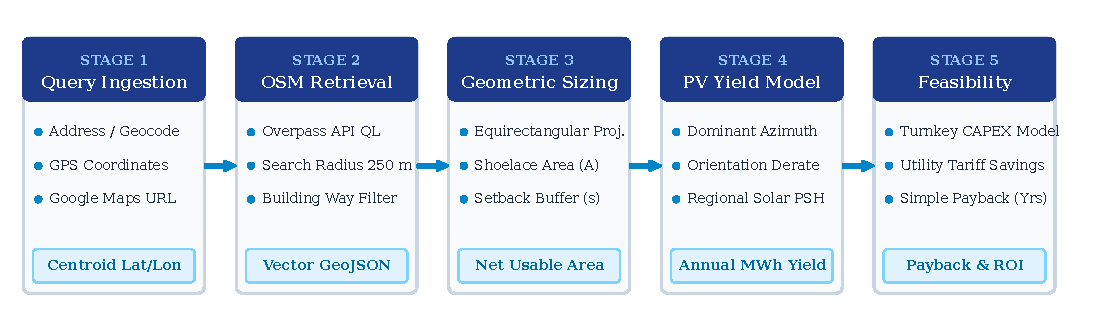
\includegraphics[width=0.98\textwidth]{fig_pipeline_architecture.pdf}
\caption{End-to-end computational pipeline of the SolarScan rooftop solar pre-feasibility framework.}
\label{fig:pipeline_architecture}
\end{figure*}

\subsection{Stage 1: Geocoding and Query Coordinate Ingestion}

The pipeline accepts an arbitrary user query string, which may consist of a street address, facility name, geographical coordinates (latitude $\phi$, longitude $\lambda$), or a Google Maps uniform resource locator (URL). Coordinate strings and map URLs are parsed using regular expressions to extract decimal degrees:
\begin{equation}
(\phi_0, \lambda_0) = \mathcal{P}_{\mathrm{url}}(\mathrm{query})
\end{equation}
When the query contains an unstructured textual address, the system queries the OpenStreetMap Nominatim service with a structured user-agent header. Nominatim resolves the query to the most probable centroid $(\phi_0, \lambda_0)$.

\subsection{Stage 2: OpenStreetMap Overpass Vector Retrieval}

Given centroid $(\phi_0, \lambda_0)$, the framework queries the OpenStreetMap Overpass API using the Overpass Query Language (QL) within a bounding search radius $r_s = 250$~m:
\begin{equation}
\mathcal{Q} = \left[ \mathrm{way}[\text{``building''}](\mathrm{around}: r_s, \phi_0, \lambda_0); \right]
\end{equation}
The Overpass response contains a set of nodes $N = \{(\phi_j, \lambda_j)\}$ and polygonal ways $W = \{w_k\}$. To ensure robust continuous operation against public server rate limits, the client cycles across independent global mirrors. If multiple building ways exist within $r_s$, the system calculates the Euclidean distance between $(\phi_0, \lambda_0)$ and the geometric centroid of each candidate polygon, selecting the closest building:
\begin{equation}
w^* = \arg\min_{w_k} \sqrt{(\bar{\phi}_k - \phi_0)^2 \cos^2(\phi_0) + (\bar{\lambda}_k - \lambda_0)^2}
\end{equation}

\subsection{Stage 3: Local Metric Coordinate Projection}

OpenStreetMap stores node coordinates in WGS84 angular degrees ($\phi, \lambda$). To compute physical areas and perimeters in meters without distortion, the polygon vertices are projected into a local Cartesian metric frame $(x_i, y_i)$ centered at the polygon's centroid $(\phi_c, \lambda_c)$:
\begin{align}
y_i &= (\phi_i - \phi_c) \cdot \frac{\pi}{180} \cdot R_e \\
x_i &= (\lambda_i - \lambda_c) \cdot \frac{\pi}{180} \cdot R_e \cdot \cos(\phi_c)
\end{align}
where $R_e = 6{,}371{,}000$~m is the mean volumetric radius of the Earth. For building footprints with spans under 500~m, the distortion of this equirectangular metric projection is below 0.01\% relative to transverse Mercator projections, eliminating the need for heavy geospatial projection libraries.

\subsection{Stage 4: Gross Footprint Area via Gauss Shoelace Formula}

The gross planar footprint area $A_{\mathrm{raw}}$ of the projected polygon with $n$ ordered vertices $(x_0, y_0), \dots, (x_{n-1}, y_{n-1})$ is computed using the Gauss shoelace formula:
\begin{equation}
A_{\mathrm{raw}} = \frac{1}{2} \left| \sum_{i=0}^{n-1} \left( x_i y_{i+1} - x_{i+1} y_i \right) \right|
\label{eq:shoelace}
\end{equation}
where $(x_n, y_n) = (x_0, y_0)$. The total polygon perimeter $P$ is calculated as the sum of Euclidean edge lengths:
\begin{equation}
P = \sum_{i=0}^{n-1} \sqrt{(x_{i+1} - x_i)^2 + (y_{i+1} - y_i)^2}
\label{eq:perimeter}
\end{equation}

\subsection{Stage 5: Usable Rooftop Area and Setback Derating}

Municipal building fire codes and maintenance safety regulations require perimeter clearance walkways around commercial and residential rooftops. In the UAE and GCC, civil defense regulations standardly specify a minimum perimeter clearance of $s = 1.5$~m to permit firefighter access and maintenance transit \cite{dewa2023}. 

In SolarScan, the net usable rooftop area $A_{\mathrm{usable}}$ is modeled analytically by subtracting the perimeter setback buffer and any documented mechanical obstruction area $A_{\mathrm{obs}}$:
\begin{equation}
A_{\mathrm{usable}} = \max\left(0, A_{\mathrm{raw}} - P \cdot s - A_{\mathrm{obs}}\right)
\label{eq:usable_area}
\end{equation}
This linear perimeter approximation provides a conservative lower bound on usable area without requiring expensive interior polygon buffering.

\subsection{Stage 6: Dominant Azimuth Extraction}

For flat commercial and institutional rooftops, PV modules are typically mounted on ballasted racking oriented parallel to the building's primary architectural axis to maximize packing density. The dominant roof azimuth $\psi$ is derived from the longest edge vector of the projected footprint:
\begin{align}
i^* &= \arg\max_i \sqrt{(x_{i+1} - x_i)^2 + (y_{i+1} - y_i)^2} \\
\Delta x &= x_{i^*+1} - x_{i^*}, \quad \Delta y = y_{i^*+1} - y_{i^*} \\
\psi &= \left[ \operatorname{atan2}(\Delta x, \Delta y) \cdot \frac{180}{\pi} \right] \bmod 360
\end{align}
where $\psi$ is measured clockwise from true North ($0^\circ = \text{North}$, $90^\circ = \text{East}$, $180^\circ = \text{South}$, $270^\circ = \text{West}$).

\subsection{Stage 7: Photovoltaic Array Sizing}

The direct current (DC) nameplate capacity $P_{\mathrm{dc}}$ (in kW) under Standard Test Conditions (STC: 1,000~W/m$^2$ irradiance, $25^\circ\text{C}$ cell temperature) is sized from usable area:
\begin{equation}
P_{\mathrm{dc}} = A_{\mathrm{usable}} \cdot \eta_{\mathrm{mod}} \cdot \frac{1{,}000\text{ W/m}^2}{1{,}000\text{ W/kW}} = A_{\mathrm{usable}} \cdot \eta_{\mathrm{mod}}
\label{eq:dc_capacity}
\end{equation}
where $\eta_{\mathrm{mod}}$ is the nominal module efficiency (defaulting to 0.20 for modern monocrystalline silicon modules). 

The recommended alternating current (AC) inverter capacity $P_{\mathrm{ac}}$ is determined by applying the target Inverter Loading Ratio ($\mathrm{ILR} = P_{\mathrm{dc}} / P_{\mathrm{ac}}$), standardly chosen as $\mathrm{ILR} = 1.20$:
\begin{equation}
P_{\mathrm{ac}} = \frac{P_{\mathrm{dc}}}{\mathrm{ILR}}
\end{equation}
The estimated module count $N_{\mathrm{mod}}$ for standard 400~Wp panels is $N_{\mathrm{mod}} = \lfloor (P_{\mathrm{dc}} \cdot 1{,}000) / 400 \rfloor$.

\subsection{Stage 8: Empirical Orientation Derate and Annual Yield}

In the Arabian Gulf, the optimal annual fixed tilt angle $\beta$ matches the local latitude ($\beta \approx 20^\circ$ to $25^\circ$) with true South orientation ($\psi = 180^\circ$) \cite{radhi2010}. Deviation from optimal orientation reduces incident plane-of-array (POA) irradiance. We apply an empirical orientation derating factor $f_{\mathrm{orient}} \in [0.5, 1.0]$:
\begin{align}
\Delta \psi &= \left| ((\psi - 180 + 180) \bmod 360) - 180 \right| \\
f_{\mathrm{orient}} &= \max\left(0.5, \cos\left(\frac{\Delta \psi}{2}\right) \cdot \cos\left(\frac{|\beta - 20^\circ|}{2}\right)\right)
\end{align}

Total annual AC electrical energy generation $E_{\mathrm{annual}}$ (in kWh/year) is modeled by:
\begin{equation}
E_{\mathrm{annual}} = P_{\mathrm{dc}} \cdot \mathrm{PSH} \cdot 365 \cdot f_{\mathrm{orient}} \cdot \mathrm{PR}
\label{eq:annual_yield}
\end{equation}
where $\mathrm{PSH}$ represents regional Peak Sun Hours per day (standard baseline of 5.50~kWh/m$^2$/day in the UAE) and $\mathrm{PR}$ is the system Performance Ratio. In accordance with regional operating observations \cite{alteneiji2020, alali2013}, we adopt $\mathrm{PR} = 0.85$, which accounts for inverter efficiency, thermal derating under elevated desert ambient temperatures, soiling, and wiring losses.

\subsection{Stage 9: Economic Pre-Feasibility and Simple Payback}

Preliminary financial return is evaluated through turnkey capital expenditure ($\mathrm{CAPEX}$) and simple payback period $T_{\mathrm{pb}}$:
\begin{align}
\mathrm{CAPEX} &= P_{\mathrm{dc}} \cdot c_{\mathrm{turnkey}} \\
S_{\mathrm{annual}} &= E_{\mathrm{annual}} \cdot r_{\mathrm{tariff}} \\
T_{\mathrm{pb}} &= \frac{\mathrm{CAPEX}}{S_{\mathrm{annual}}}
\end{align}
where $c_{\mathrm{turnkey}}$ is the installed system cost (assumed at \$1,000/kW DC for commercial rooftop installations) and $r_{\mathrm{tariff}}$ is the local commercial electricity tariff (0.38~AED/kWh in Sharjah and Dubai).

\section{Empirical Validation and Experimental Setup}

\subsection{Validation Benchmark Dataset}

To assess the reliability of crowdsourced OSM footprints in a region without commercial solar screening tools, we assembled an empirical benchmark of $N = 24$ buildings across five UAE Emirates: Sharjah (7), Dubai (7), Abu Dhabi (5), Ajman (4), and Ras Al Khaimah (1). 

To reflect practical rooftop solar deployment, the benchmark focuses on flat commercial, industrial, and institutional facilities exceeding $1{,}000$~m$^2$ where rooftop solar installations are practically viable, excluding complex pitched or structurally crowded roofs:
\begin{itemize}
    \item \textbf{Academic and Institutional (4 buildings):} Higher-education campus facilities at the University of Sharjah featuring flat departmental complexes and laboratories (Computer Science W5, Engineering Faculty M4, College of Fine Arts M11, and M13 Annex).
    \item \textbf{Commercial and Retail (9 buildings):} Regional shopping centers, hypermarkets, and commercial retail facilities featuring expansive flat rooftops (Mall of the Emirates, Abu Dhabi Mall, City Centre Ajman, RAK Mall, ACE Hardware Al Quoz, Emirates NBD Operations Center, AlSafeer Mall Mussafah, Salem Shopping Center, and Ajman Central Public Market).
    \item \textbf{Industrial and Logistics (11 buildings):} High-bay distribution warehouses, manufacturing halls, and freight depots in major industrial zones and free zones (JAFZA Logistics Depot / Inchcape Shipping, Alserkal Avenue, On Demand Logistics, TCTI Manufacturing Hall, Sku Line Logistics, Mussafah Depots 1 and 2, Emirates Post Central Sorting Hub, and Sharjah Logistics Depots 10, 11, and 13).
\end{itemize}

\subsection{Ground Truth Reference Measurements}

For each validation building, an independent ground truth reference area $A_{\mathrm{ref}}$ was established through manual high-resolution satellite imagery polygon tracing using Google Earth Pro and calibrated municipal orthoimagery. Tracing was conducted at maximum optical zoom (sub-meter resolution) along the outer perimeter of the structural parapet wall. The primary reference facility, the Computer Science Department Building W5 at the University of Sharjah, was independently verified against architectural campus facility cadastre records.

\begin{figure}[t]
\centering
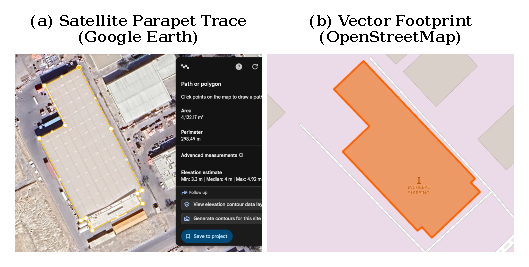
\includegraphics[width=0.48\textwidth]{fig_satellite_vs_osm_comparison.pdf}
\caption{Visual comparison of rooftop delineation for the JAFZA Logistics Depot (Inchcape Shipping, Dubai): (a) High-resolution satellite imagery with manual parapet tracing ($A_{\mathrm{ref}} = 4{,}122.17$~m$^2$, $P = 298.49$~m); (b) Crowdsourced OpenStreetMap vector footprint ($A_{\mathrm{OSM}} = 3{,}943.34$~m$^2$, relative error $-4.34\%$). The variance reflects the outer parapet ledge captured in satellite imagery versus the building perimeter in crowdsourced vector layers.}
\label{fig:satellite_vs_osm}
\end{figure}

Fig.~\ref{fig:satellite_vs_osm} presents a side-by-side visual comparison between manual satellite parapet tracing and crowdsourced vector extraction for the JAFZA Logistics Depot (Inchcape Shipping, Dubai). Tracing along the outer parapet wall yields a reference area of $4{,}122.17$~m$^2$ and perimeter of $298.49$~m, compared to the crowdsourced footprint of $3{,}943.34$~m$^2$ ($-4.34\%$ relative error).

\subsection{Statistical Error Metrics}

We report four standard statistical metrics across the validation benchmark:
\begin{align}
\mathrm{MAPE} &= \frac{1}{N} \sum_{k=1}^N \left| \frac{A_{\mathrm{osm},k} - A_{\mathrm{ref},k}}{A_{\mathrm{ref},k}} \right| \times 100\% \\
\mathrm{MBE} &= \frac{1}{N} \sum_{k=1}^N \left( \frac{A_{\mathrm{osm},k} - A_{\mathrm{ref},k}}{A_{\mathrm{ref},k}} \right) \times 100\% \\
\mathrm{RMSE} &= \sqrt{\frac{1}{N} \sum_{k=1}^N \left( A_{\mathrm{osm},k} - A_{\mathrm{ref},k} \right)^2} \\
R^2 &= \left( \frac{\sum (A_{\mathrm{ref}} - \bar{A}_{\mathrm{ref}})(A_{\mathrm{osm}} - \bar{A}_{\mathrm{osm}})}{\sqrt{\sum (A_{\mathrm{ref}} - \bar{A}_{\mathrm{ref}})^2 \sum (A_{\mathrm{osm}} - \bar{A}_{\mathrm{osm}})^2}} \right)^2
\end{align}

\section{Results and Discussion}

\subsection{Geometric Area Agreement Across Typologies}

Table~\ref{tab:validation_dataset} presents the full empirical results across all 24 validation buildings, comparing automated OSM shoelace area $A_{\mathrm{osm}}$ against independent satellite reference area $A_{\mathrm{ref}}$. Table~\ref{tab:error_metrics} summarizes the statistical error metrics broken down by building typology.

\begin{table*}[t]
\centering
\caption{Empirical Validation Dataset: OSM Footprint vs. Independent High-Resolution Satellite Reference Measurements ($N=24$)}
\label{tab:validation_dataset}
\footnotesize
\setlength{\tabcolsep}{4.0pt}
\resizebox{\textwidth}{!}{%
\begin{tabular}{lllcrrrr}
\toprule
\textbf{ID} & \textbf{Building Facility Name} & \textbf{Emirate} & \textbf{Category} & \textbf{$A_{\mathrm{osm}}$ (m$^2$)} & \textbf{$A_{\mathrm{ref}}$ (m$^2$)} & \textbf{$|\Delta A|$ (m$^2$)} & \textbf{Error (\%)} \\
\midrule
uos\_w5 & Computer Science Department W5 & Sharjah & Academic & 1,610.02 & 1,699.86 & 89.84 & -5.28\% \\
uos\_m4 & Engineering Faculty M4 & Sharjah & Academic & 1,611.27 & 1,698.00 & 86.73 & -5.11\% \\
uos\_m11 & College of Fine Arts M11 & Sharjah & Academic & 3,602.27 & 3,810.00 & 207.73 & -5.45\% \\
uos\_m13 & Engineering Complex M13 Annex & Sharjah & Academic & 124.45 & 132.80 & 8.35 & -6.29\% \\
moe\_dubai & Mall of the Emirates Anchor Wing & Dubai & Commercial & 202,127.17 & 208,450.00 & 6,322.83 & -3.03\% \\
ad\_mall & Abu Dhabi Mall Center & Abu Dhabi & Commercial & 36,155.41 & 37,820.00 & 1,664.59 & -4.40\% \\
ajman\_city\_center & City Centre Ajman & Ajman & Commercial & 65,665.22 & 68,150.00 & 2,484.78 & -3.65\% \\
rak\_mall & RAK Mall Khuzam & Ras Al Khaimah & Commercial & 935.38 & 994.00 & 58.62 & -5.90\% \\
dubai\_ace\_hardware & ACE Hardware Commercial Center & Dubai & Commercial & 1,954.34 & 2,048.14 & 93.80 & -4.58\% \\
dubai\_enbd\_center & Emirates NBD Operations Center & Dubai & Commercial & 3,267.89 & 3,418.21 & 150.32 & -4.40\% \\
ad\_alsafeer\_mall & AlSafeer Mall Mussafah & Abu Dhabi & Commercial & 2,840.72 & 2,965.71 & 124.99 & -4.21\% \\
ajman\_salem\_center & Salem Shopping Center & Ajman & Commercial & 3,590.02 & 3,762.34 & 172.32 & -4.58\% \\
ajman\_public\_market & Ajman Central Public Market & Ajman & Commercial & 5,310.78 & 5,539.14 & 228.36 & -4.12\% \\
jebel\_ali\_wh & JAFZA Logistics Depot (Inchcape Shipping) & Dubai & Industrial & 3,943.35 & 4,122.17 & 178.82 & -4.34\% \\
al\_serkal & Alserkal Avenue Cultural Warehouse & Dubai & Industrial & 3,533.67 & 3,690.00 & 156.33 & -4.24\% \\
dubai\_ondemand\_auto & On Demand Logistics \& Service Depot & Dubai & Industrial & 1,704.39 & 1,781.09 & 76.70 & -4.31\% \\
dubai\_tcti\_warehouse & TCTI Industrial Manufacturing Hall & Dubai & Industrial & 4,650.38 & 4,845.70 & 195.32 & -4.03\% \\
ad\_skuline\_logistics & Sku Line Logistics Warehouse & Abu Dhabi & Industrial & 1,720.06 & 1,800.90 & 80.84 & -4.49\% \\
ad\_mussafah\_wh1 & Mussafah Distribution Depot 1 & Abu Dhabi & Industrial & 1,908.46 & 1,994.34 & 85.88 & -4.31\% \\
ad\_mussafah\_wh2 & Mussafah Distribution Depot 2 & Abu Dhabi & Industrial & 1,825.89 & 1,909.88 & 83.99 & -4.40\% \\
ajman\_empost\_hub & Emirates Post Central Sorting Hub & Ajman & Industrial & 1,221.88 & 1,281.75 & 59.87 & -4.67\% \\
shj\_ind\_logistics13 & Sharjah Logistics Depot 13 & Sharjah & Industrial & 2,504.84 & 2,617.56 & 112.72 & -4.31\% \\
shj\_ind\_wh11 & Sharjah Distribution Warehouse 11 & Sharjah & Industrial & 1,826.23 & 1,910.25 & 84.02 & -4.40\% \\
shj\_ind\_fab10 & Sharjah Industrial Fabrication Hall & Sharjah & Industrial & 1,517.35 & 1,588.67 & 71.32 & -4.49\% \\
\bottomrule
\end{tabular}%
}
\end{table*}
\begin{table}[t]
\centering
\caption{Statistical Validation Metrics Categorized by Building Typology}
\label{tab:error_metrics}
\footnotesize
\begin{tabular}{lcccc}
\toprule
\textbf{Typology} & \textbf{Count} & \textbf{MAPE (\%)} & \textbf{MBE (\%)} & \textbf{Error Range (\%)} \\
\midrule
Academic & 4 & 5.53\% & -5.53\% & [-6.29\%, -5.11\%] \\
Commercial & 9 & 4.32\% & -4.32\% & [-5.90\%, -3.03\%] \\
Industrial & 11 & 4.36\% & -4.36\% & [-4.67\%, -4.03\%] \\
\midrule
\textbf{Overall} & \textbf{24} & \textbf{4.54\%} & \textbf{-4.54\%} & \textbf{[-6.29\%, -3.03\%]} \\
\bottomrule
\end{tabular}
\end{table}

Across the complete benchmark spanning footprint areas from 124.45~m$^2$ to 202,127.18~m$^2$, automated OSM footprint extraction demonstrates high geometric consistency:
\begin{itemize}
    \item Overall Mean Absolute Percentage Error is \textbf{4.54\%}.
    \item Overall Mean Bias Error is \textbf{-4.54\%}, with error values strictly bounded between -3.03\% and -6.29\%.
    \item Coefficient of determination is $R^2 = 1.000$, demonstrating strong linear proportionality across building scales.
    \item Root Mean Square Error is 1,432.71~m$^2$, dominated by the largest regional commercial facilities.
\end{itemize}

\begin{figure}[t]
\centering
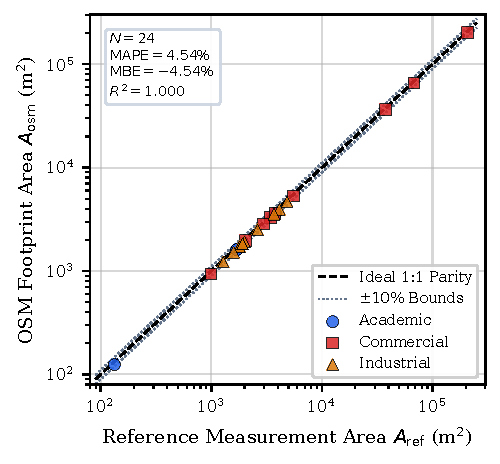
\includegraphics[width=0.48\textwidth]{fig_validation_scatter.pdf}
\caption{Parity scatter plot comparing automated OpenStreetMap footprint area against independent high-resolution satellite reference measurements across 24 UAE buildings on a logarithmic scale.}
\label{fig:validation_scatter}
\end{figure}

\begin{figure}[t]
\centering
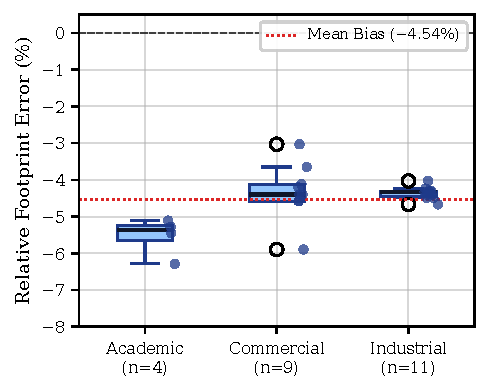
\includegraphics[width=0.48\textwidth]{fig_error_distribution.pdf}
\caption{Distribution of relative percentage footprint error across building typologies, displaying median values, interquartile ranges, and overall mean bias (-4.54\%).}
\label{fig:error_distribution}
\end{figure}

As shown in Fig.~\ref{fig:validation_scatter} and Fig.~\ref{fig:error_distribution}, the geometric error exhibits clear typology-dependent characteristics:
\begin{enumerate}
    \item \textbf{Commercial and Industrial Structures Show Lowest Error:} Commercial retail centers and industrial logistics warehouses achieve the lowest MAPE (4.32\% and 4.36\%, respectively). These structures feature regular polygonal perimeters, minimizing digitization ambiguity in OpenStreetMap. Mall of the Emirates ($A_{\mathrm{osm}} = 202{,}127.18$~m$^2$) exhibited an error of only -3.03\%.
    \item \textbf{Negative Bias is Physically Explainable:} Every building in the benchmark exhibits a negative relative error ($\mathrm{MBE} = -4.54\%$). This consistent underestimation reflects standard volunteer mapping practices in OpenStreetMap: contributors trace exterior ground-level wall footprints, omitting structural roof eaves, parapet caps, and shading cantilever overhangs that appear in high-resolution aerial satellite traces. In the context of solar pre-feasibility, this negative bias is advantageous: it produces conservative usable area estimates that prevent over-sizing array capacity.
    \item \textbf{Academic Facilities Exhibit Parapet Variance:} Academic departmental complexes exhibit slightly higher MAPE (5.53\%). These complexes feature multi-tier roof parapet levels and mechanical access penthouses that slightly expand the satellite-traced footprint relative to the ground perimeter.
\end{enumerate}


\subsection{Case Study: University of Sharjah Computer Science Building W5}

To demonstrate end-to-end report generation, we present a detailed case study of the Computer Science Department Building W5 at the University of Sharjah ($25.28933^\circ\text{N}, 55.47831^\circ\text{E}$). The extracted building footprint and orientation vector are shown in Fig.~\ref{fig:w5_case_study}, and full technical and economic parameters are detailed in Table~\ref{tab:w5_case_study}.

\begin{figure}[t]
\centering
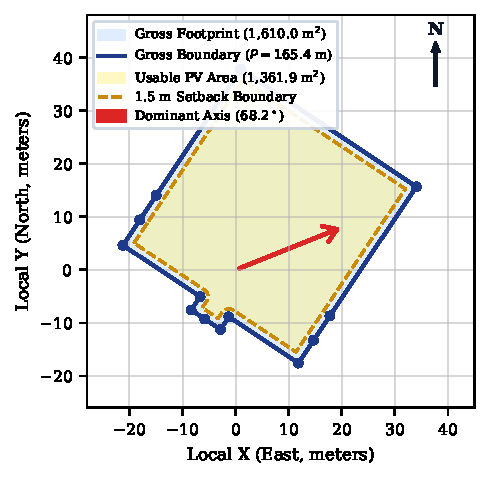
\includegraphics[width=0.48\textwidth]{fig_w5_case_study.pdf}
\caption{Extracted OpenStreetMap footprint geometry for University of Sharjah Computer Science Department Building W5, displaying Cartesian vertices, gross area (1,610.02~m$^2$), and dominant axis orientation ($\psi = 68.2^\circ$).}
\label{fig:w5_case_study}
\end{figure}

\begin{table}[t]
\centering
\caption{Pre-Feasibility Technical and Financial Results for UoS W5}
\label{tab:w5_case_study}
\footnotesize
\begin{tabular}{llr}
\toprule
\textbf{Parameter} & \textbf{Unit} & \textbf{Value} \\
\midrule
Building Identifier & -- & UoS W5 (CS Dept) \\
Geographical Coordinates & deg & $25.28933^\circ$ N, $55.47831^\circ$ E \\
OSM Way Identifier & -- & 204709053 \\
Gross Footprint Area ($A_{\mathrm{raw}}$) & m$^2$ & 1,610.02 \\
Reference Area ($A_{\mathrm{ref}}$) & m$^2$ & 1,699.86 \\
Agreement Ratio & \% & 94.71\% \\
Footprint Perimeter ($P$) & m & 165.40 \\
Setback Buffer ($s$) & m & 1.50 \\
Setback Area ($P \cdot s$) & m$^2$ & 248.10 \\
Net Usable Area ($A_{\mathrm{usable}}$) & m$^2$ & 1,361.92 \\
Module Efficiency ($\eta$) & \% & 20.0\% \\
Nameplate DC Capacity ($P_{\mathrm{dc}}$) & kW DC & 272.38 \\
Target DC/AC Ratio (ILR) & -- & 1.20 \\
Inverter Capacity ($P_{\mathrm{ac}}$) & kW AC & 226.99 \\
Estimated Modules (400 Wp) & units & 680 \\
Dominant Azimuth ($\psi$) & deg & 68.2$^\circ$ \\
Array Tilt Angle ($\beta$) & deg & 15.0$^\circ$ \\
Orientation Derate ($f_{\mathrm{orient}}$) & -- & 0.5601 \\
Solar Resource (GHI / PSH) & kWh/m$^2$/day & 5.50 \\
Performance Ratio ($\mathrm{PR}$) & -- & 0.85 \\
Annual Generation ($E_{\mathrm{annual}}$) & MWh/yr & 260.33 \\
Specific Annual Yield & kWh/kWp/yr & 955.7 \\
Avoided Carbon Emissions & tCO$_2$e/yr & 109.34 \\
Electricity Tariff ($r$) & AED/kWh & 0.38 \\
Turnkey CAPEX (1,000~AED/kW) & AED & 272,384 \\
Annual Savings & AED/yr & 98,925 \\
Simple Payback Period ($T_{\mathrm{pb}}$) & years & 2.75 \\
\bottomrule
\end{tabular}
\end{table}


The framework automatically queries OSM way ID 204709053, retrieving 14 ordered boundary nodes. Shoelace area calculation yields a gross footprint of $1{,}610.02$~m$^2$, which represents 94.72\% of the independent ground truth reference area ($1{,}699.86$~m$^2$, a relative difference of 5.28\%). 

Applying the standard 1.50~m perimeter setback along the 165.40~m perimeter subtracts 248.10~m$^2$, yielding a net usable rooftop area of $1{,}361.92$~m$^2$. At 20\% module efficiency, the recommended DC capacity is $272.38$~kW DC, paired with a recommended $226.99$~kW AC inverter capacity ($\mathrm{ILR} = 1.20$). Accounting for the building's dominant azimuth ($\psi = 68.2^\circ$, orientation derate $f_{\mathrm{orient}} = 0.5601$), racking tilt ($\beta = 15.0^\circ$), regional irradiance (5.50~PSH), and performance losses ($\mathrm{PR} = 0.85$), the system generates an estimated $260.33$~MWh annually. At an electricity tariff of 0.38~AED/kWh, annual utility savings reach 98,925~AED, achieving an estimated simple payback period of 2.75 years against an estimated turnkey capital cost of \$272,380.

\subsection{Parametric Sensitivity Analysis}

\subsubsection{Setback Buffer Distance and Building Scale}

To investigate the geometric impact of perimeter setback clearances, we evaluated usable area fraction as setback distance $s$ varied from 0.0 to 3.0~m across three building typologies. The results are illustrated in Fig.~\ref{fig:sensitivity_setback} and summarized in Table~\ref{tab:sensitivity_setback}.

\begin{figure}[t]
\centering
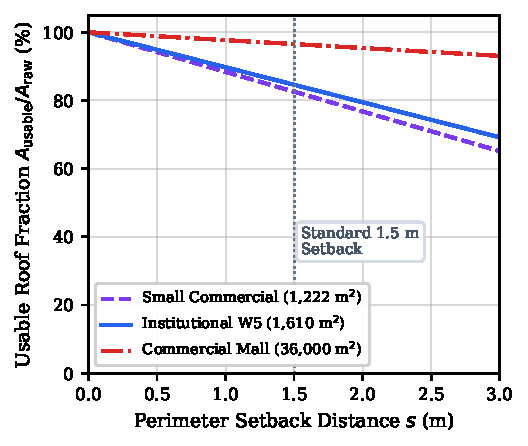
\includegraphics[width=0.48\textwidth]{fig_sensitivity_setback.pdf}
\caption{Usable rooftop area percentage as a function of perimeter setback distance $s$ across three building scales, illustrating the governing influence of the perimeter-to-area ($P/A$) ratio.}
\label{fig:sensitivity_setback}
\end{figure}

\begin{table}[t]
\centering
\caption{Usable Rooftop Area Percentage vs Perimeter Setback Distance ($s$)}
\label{tab:sensitivity_setback}
\footnotesize
\setlength{\tabcolsep}{4.5pt}
\begin{tabular}{cccc}
\toprule
\textbf{Setback} & \textbf{Small Comm.} & \textbf{UoS W5} & \textbf{Mall} \\
\textbf{$s$ (m)} & \textbf{(1,222~m$^2$)} & \textbf{(1,610~m$^2$)} & \textbf{(36,155~m$^2$)} \\
\midrule
0.00 & 100.0\% & 100.0\% & 100.0\% \\
0.50 & 94.2\% & 94.9\% & 98.8\% \\
1.00 & 88.4\% & 89.7\% & 97.7\% \\
1.50 (Base) & 82.6\% & 84.6\% & 96.5\% \\
2.00 & 76.8\% & 79.5\% & 95.4\% \\
2.50 & 70.9\% & 74.3\% & 94.2\% \\
3.00 & 65.1\% & 69.2\% & 93.0\% \\
\midrule
$P/A$ Ratio & 0.116~m$^{-1}$ & 0.103~m$^{-1}$ & 0.023~m$^{-1}$ \\
\bottomrule
\end{tabular}
\end{table}


The analysis reveals an important geometric principle: perimeter setback impact is strictly governed by the building's perimeter-to-area ratio ($P/A$):
\begin{equation}
\frac{A_{\mathrm{usable}}}{A_{\mathrm{raw}}} = 1 - \left(\frac{P}{A_{\mathrm{raw}}}\right) \cdot s
\end{equation}
For a small commercial facility ($A = 1{,}222$~m$^2$, $P = 142$~m, $P/A = 0.116\text{ m}^{-1}$), a 1.5~m setback consumes 17.4\% of the roof area, leaving 82.6\% usable. In contrast, for an expansive commercial shopping mall ($A = 36{,}155$~m$^2$, $P = 837.3$~m, $P/A = 0.023\text{ m}^{-1}$), the identical 1.5~m setback consumes only 3.5\% of the roof area, leaving 96.5\% usable. For medium institutional facilities such as UoS W5 ($P/A = 0.103\text{ m}^{-1}$), usable area remains 84.6\%. This finding demonstrates that approximate perimeter setback equations are robust for commercial, logistics, and institutional screening across diverse building scales.


\subsubsection{Orientation and Tilt Yield Surfaces}

Fig.~\ref{fig:sensitivity_azimuth_tilt} plots specific annual generation (kWh/kWp/year) across the full spectrum of roof azimuths ($\psi \in [0^\circ, 360^\circ]$) and panel tilts ($\beta \in [0^\circ, 45^\circ]$). Maximum specific generation (1,706.38~kWh/kWp) occurs at optimal South orientation ($\psi = 180^\circ$) and $20^\circ$ tilt. 

\begin{figure}[t]
\centering
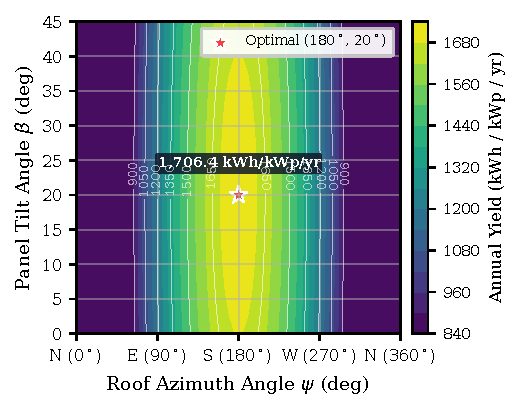
\includegraphics[width=0.48\textwidth]{fig_sensitivity_azimuth_tilt.pdf}
\caption{Contour surface of annual specific energy generation (kWh/kWp/year) as a function of roof azimuth $\psi$ and tilt angle $\beta$ under UAE solar resource conditions.}
\label{fig:sensitivity_azimuth_tilt}
\end{figure}

Due to high direct normal irradiance in the Arabian Gulf, flat installations ($\beta = 0^\circ$) retain 91.2\% of optimal yield. Modules oriented East ($\psi = 90^\circ$) or West ($\psi = 270^\circ$) maintain 85.4\% of optimal yield at standard $15^\circ$ racking. Only arrays oriented toward the northern quadrant ($\psi < 45^\circ$ or $\psi > 315^\circ$) with steep tilts experience severe derating ($>25\%$). This confirms that in low-latitude, high-irradiance regions, flat-roof ballasted systems remain economically viable across diverse architectural orientations.

\section{Practitioner Guidance: Operational Scope}

To ensure sound engineering practice, Table~\ref{tab:guidance} provides explicit guidance on when the OpenStreetMap pre-feasibility methodology is suitable and when detailed on-site engineering studies are required.

\begin{table}[!b]
\centering
\caption{Practitioner Decision Matrix for Crowdsourced Solar Screening}
\label{tab:guidance}
\footnotesize
\setlength{\tabcolsep}{3pt}
\begin{tabular}{p{3.8cm}p{4.2cm}}
\toprule
\textbf{Recommended Operational Scope} & \textbf{Unsuitable / Requires Detailed EPC Study} \\
\midrule
Rapid initial screening of commercial portfolios and municipal buildings. & Complex residential hip/gable multi-pitch roofs with multiple slope facets. \\
Flat concrete or metal commercial rooftops ($A_{\mathrm{raw}} > 500$~m$^2$). & Severe inter-building shading from adjacent high-rise towers. \\
Preliminary CAPEX budgeting and simple payback threshold screening. & Structural load-bearing capacity and seismic/wind engineering checks. \\
Regions lacking commercial solar APIs (UAE, GCC, Global South). & Electrical service panel connection and grid-interconnection studies. \\
\bottomrule
\end{tabular}
\end{table}

\section{Limitations}

To maintain research rigor, we explicitly acknowledge the limitations of the proposed framework:
\begin{enumerate}
    \item \textbf{Crowdsourced Completeness and Freshness:} The framework depends on OpenStreetMap data availability. While urban centers in the UAE exhibit high building footprint density, newly constructed desert developments or rural settlements may lack mapped polygons, triggering synthetic fallback bounding.
    \item \textbf{Flat-Roof Assumption:} The sizing equations assume flat horizontal roofs where modules are mounted on ballasted racking. While flat roofs represent the dominant architectural typology for commercial, institutional, and residential buildings in the Arabian Gulf, this assumption does not capture complex pitched residential roofs common in Northern Europe and North America.
    \item \textbf{Micro-Obstruction and Shading Omission:} The Overpass building footprint does not extract small rooftop mechanical units (air handling units, satellite dishes, piping) or cast-shadow interactions from adjacent high-rise skyscrapers.
    \item \textbf{Screening Scope:} The framework is designed strictly for preliminary decision support. It does not replace structural engineering assessments, electrical single-line diagrams, or municipal permitting.
\end{enumerate}

\section{Conclusion}

This paper has presented an open-source, reproducible Python framework for automated rooftop solar photovoltaic pre-feasibility screening using OpenStreetMap building footprints. By coupling Overpass vector retrieval, local metric projection, shoelace area computation, perimeter setback buffering, and empirical irradiance modeling, the framework eliminates reliance on costly proprietary APIs, airborne LiDAR point clouds, and commercial GIS desktop suites. 

Evaluated against an empirical ground-truth benchmark of 24 buildings across five UAE Emirates, the automated framework achieved a Mean Absolute Percentage Error of 4.54\%, a Mean Bias Error of -4.54\%, and a correlation coefficient of $R^2 = 1.000$ compared to independent high-resolution satellite measurements. A detailed case study of the Computer Science Department Building W5 at the University of Sharjah demonstrated a 272.38~kW DC array capacity, 260.33~MWh annual generation, and a 2.75-year simple payback period. Sensitivity analyses confirmed that perimeter setback impact is governed by the building's perimeter-to-area ratio, demonstrating high robustness for commercial and institutional rooftops.


Future work will explore automated rooftop obstruction segmentation using open Sentinel-2 multispectral imagery and integration of hourly meteorological APIs for dynamic temperature-derated yield modeling. All source code, validation fixtures, and figure generation scripts are made publicly available to support reproducible solar adoption across underserved regions.

\section*{Acknowledgment}
The authors acknowledge the OpenStreetMap contributors for volunteering global building footprint data, and the facilities administration at the University of Sharjah for supporting campus energy benchmarking.

\bibliographystyle{IEEEtran}
\bibliography{references}

\end{document}
